\documentclass[border=1mm]{standalone}

\usepackage{amsmath}
\usepackage{xcolor}
\definecolor{den-6}{HTML}{666666}
\usepackage{tkz-tab}
\usetikzlibrary{arrows}

\begin{document}

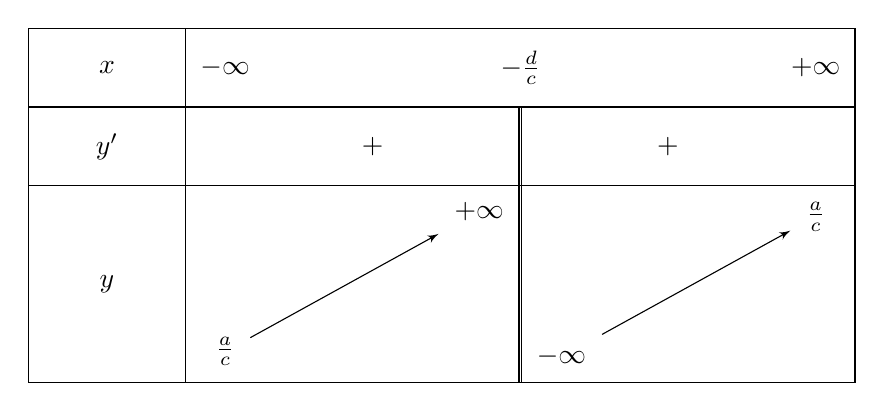
\begin{tikzpicture}

  \tkzTabInit[
    lgt=2, 
    deltacl=.5, 
    espcl=3.75]
    {$x$/1, $y^\prime$/1, $y$/2.5}
    {$-\infty$, $-\frac{d}{c}$, $+\infty$}
  \tkzTabLine{, +, d, +, } 
  \tkzTabVar{-/$\frac{a}{c}$, +D- /$+\infty$/$-\infty$, +/$\frac{a}{c}$}
  % \tkzTabVal[draw]{2}{3}{0.5}{$-\frac{1}{2}$}{$\frac{1}{2}$}
  
\end{tikzpicture}

\end{document}
